\documentclass{report}
\usepackage{homework}
\solstrue

\graphicspath{{images/}}

\renewcommand{\hmwkTitle}{Homework 6}

\begin{document}
\mktitle


\begin{problem}

Suppose an application generates chunks of 40 bytes of data, each chunk gets encapsulated in a TCP segment, and then an IP datagram.

\begin{enumerate}
\item What percentage of each datagram will be overhead, and what percentage will be application data?

\item What would be the overhead if each TCP segment include 100 of application chunks (i.e., $100 \times 40$ bytes), assuming the maximum size of an IP packet is 500 bytes and sending such big TCP payload would require fragmentation.
\end{enumerate}


\begin{answer}{40em}
  \begin{enumerate}
    \item There's 20 bytes of header information in the IP packet and 40 bytes
          of data, for a total message size of 60 bytes. 33.3\% of each packet
          will be overhead (the header) and 66.6\% application data.

    \item We would need to send 9 packets to deliver 4000 bytes of data, fitting
          480 bytes of data in each IP packet as the header takes 20 bytes of
          space in each packet. After the 9 packets are delivered, we have sent
          180 bytes of IP headers and 4000 bytes of application data. The
          overhead in this delivery is 4.3\%, and application data accounted for
          95.7\% of all bytes sent over the network.
  \end{enumerate}
\end{answer}

\end{problem}


\clearpage
\begin{problem}

Consider the router trying to send the following IP packet:

\begin{figure}[!h]
\center
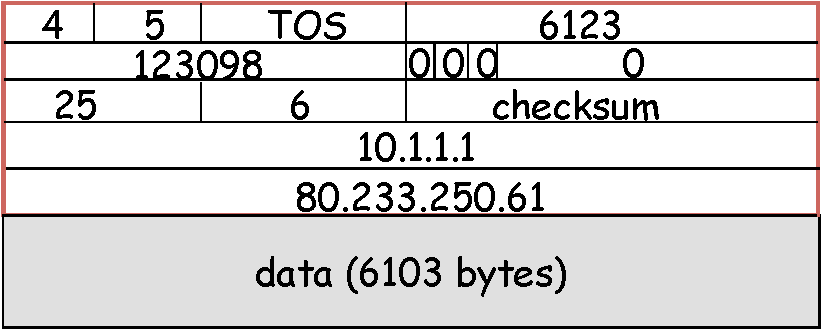
\includegraphics[scale=0.8]{hw6-frag}
\caption{An IP packet.}
\label{fig:ip-frag}
\end{figure}

Assuming that the maximum transmission unit that can be transferred over the link is 1500 bytes, show

For each of the fragment show the header length, total length, identification, flags, fragment offset, TTL, protocol fields, and IP payload size.

\vspace{20px}

\begin{tabular}[h]{|c|c|c|c|c|c|c|c|}
  \hline
  Header length &
  Total length &
  Identification &
  Flags &
  Fragment offset &
  TTL &
  Protocol &
  Data size \\
  \hline
  20 & 1500 & 123098 & 0 0 1 & 0    & 25 & 6 (TCP) & 1480 \\
  20 & 1500 & 123098 & 0 0 1 & 1480 & 25 & 6 (TCP) & 1480 \\
  20 & 1500 & 123098 & 0 0 1 & 2960 & 25 & 6 (TCP) & 1480 \\
  20 & 1500 & 123098 & 0 0 1 & 4440 & 25 & 6 (TCP) & 1480 \\
  20 & 203  & 123098 & 0 0 0 & 5920 & 25 & 6 (TCP) & 183  \\
  \hline
\end{tabular}


\end{problem}



\clearpage
\begin{problem}
Calculate the network mask, the number of bits of the network, the number of endpoint adresses in the network (excluding special addresses), the network address, and the broadcast address of the network for the following:

\begin{enumerate}
\item 131.179.196.0/24
\item 169.232.34.48/30
\item 196.22.136.0/21
\item 93.181.192.0, netmask 255.255.224.0
\item 10.128.0.0, netmask 255.192.0.0
\end{enumerate}


\begin{answer}{30em}
  \begin{enumerate}
    \item network mask: 255.255.255.0\\
          network bits: 24\\
          endpoint addresses: 254\\
          network address: 131.179.196.0\\
          broadcast address: 131.179.196.255

    \item network mask: 255.255.255.252\\
          network bits: 30\\
          endpoint addresses: 2\\
          network address: 169.232.34.48\\
          broadcast address: 169.232.34.51

    \item network mask: 255.255.248.0\\
          network bits: 21\\
          endpoint addresses: 2045\\
          network address: 196.22.136.0\\
          broadcast address: 196.22.143.255

    \item network mask: 255.255.224.0\\
          network bits: 19\\
          endpoint addresses: 8189\\
          network address: 93.181.192.0\\
          broadcast address: 93.181.223.255

    \item network mask: 255.192.0.0\\
          network bits: 10\\
          endpoint addresses: 4.194301e6\\
          network address: 10.128.0.0\\
          broadcast address: 10.191.255.255
  \end{enumerate}
\end{answer}

\end{problem}


\clearpage
\begin{problem}

Consider a simple network with one WiFi router and 3 hosts on the Figure.  Host A and B are connected to the router over wireless interface, host C is connected using wired Ethernet interface.


\begin{enumerate}
\item Assign IP (IPv4) addresses, network masks, and next hop gateways (where applicable) addresses so that all of them can communicate with each other.

Consider that have been given 131.179.196.32/27 address block and all assignments should be made from that block.   \textbf{Your assignment must use the most conservative IP address allocation.}

\item Fill the content of the Host C's routing table, \textbf{without using the default route}.
\end{enumerate}

\vspace{1cm}

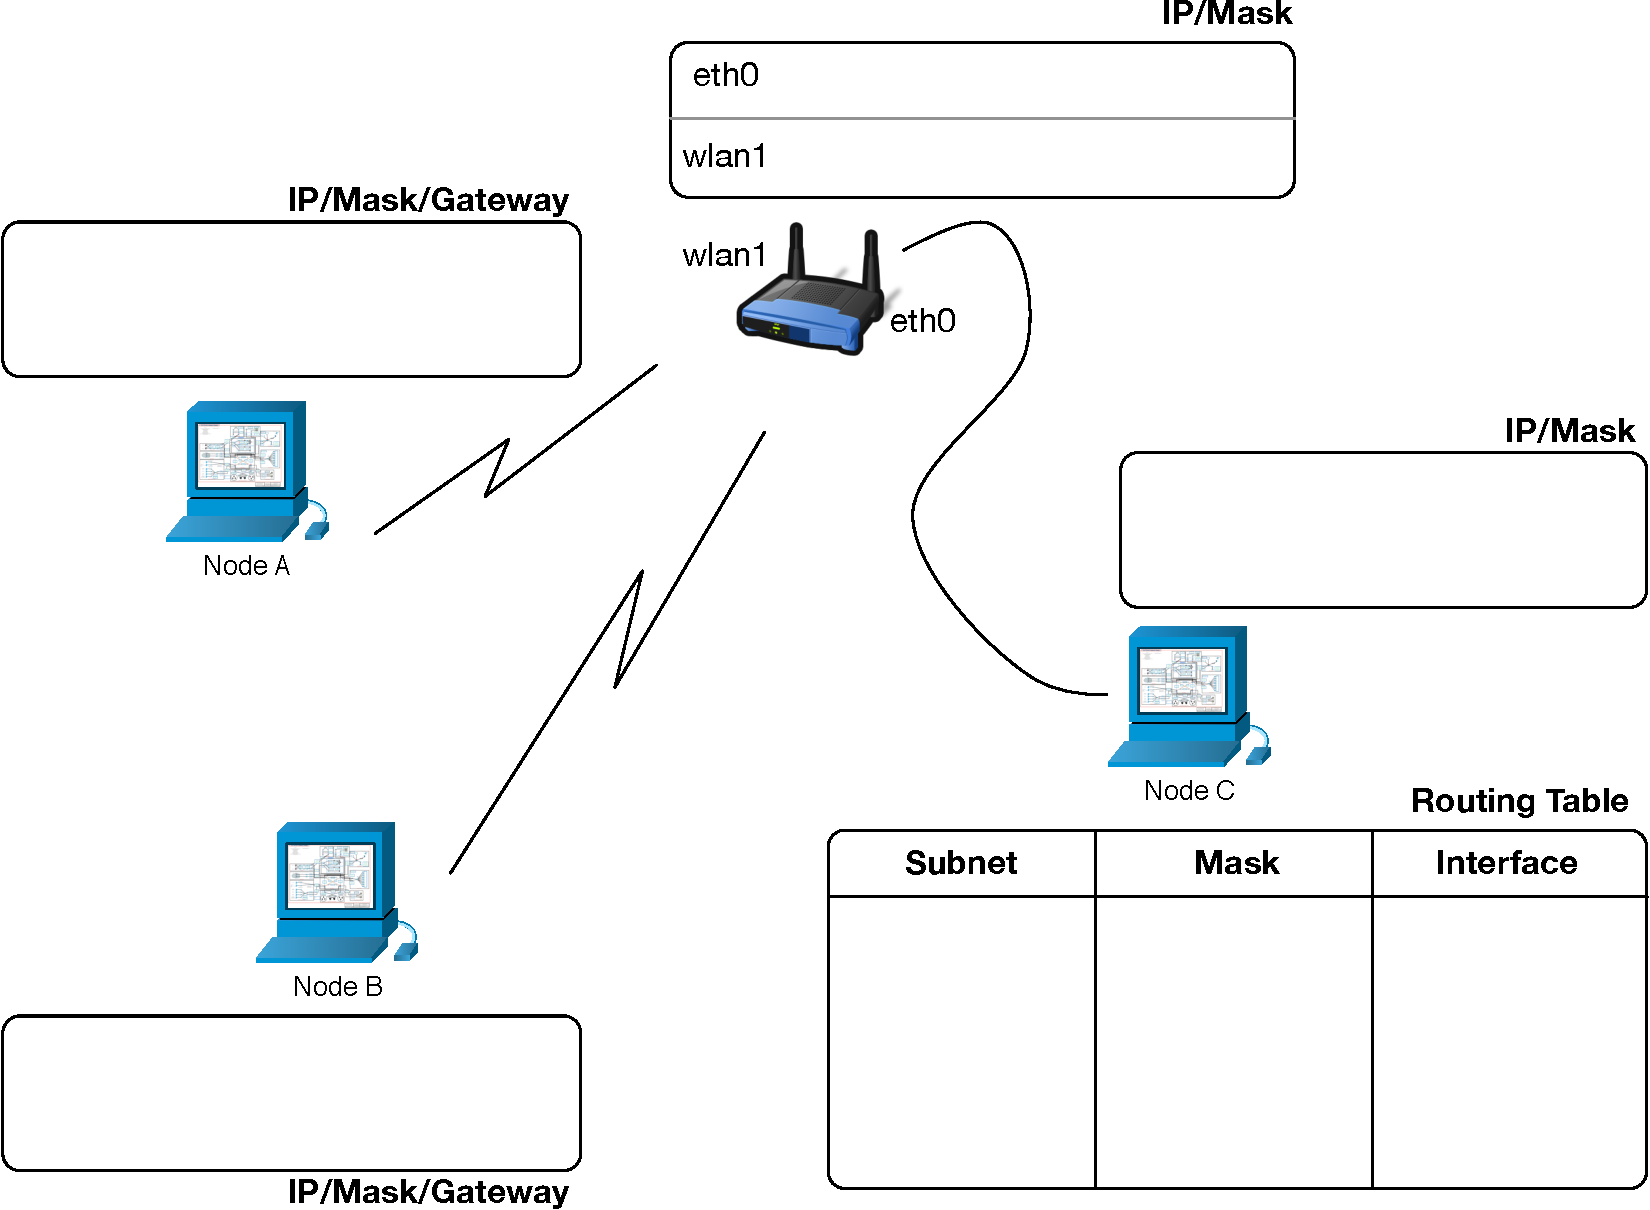
\includegraphics[scale=0.6]{hw6-topo}

\end{problem}



\end{document}
